
\documentclass[11pt,oneside, a4paper]{amsart}\usepackage[]{graphicx}\usepackage[]{color}
%% maxwidth is the original width if it is less than linewidth
%% otherwise use linewidth (to make sure the graphics do not exceed the margin)
\makeatletter
\def\maxwidth{ %
  \ifdim\Gin@nat@width>\linewidth
    \linewidth
  \else
    \Gin@nat@width
  \fi
}
\makeatother

\definecolor{fgcolor}{rgb}{0.345, 0.345, 0.345}
\newcommand{\hlnum}[1]{\textcolor[rgb]{0.686,0.059,0.569}{#1}}%
\newcommand{\hlstr}[1]{\textcolor[rgb]{0.192,0.494,0.8}{#1}}%
\newcommand{\hlcom}[1]{\textcolor[rgb]{0.678,0.584,0.686}{\textit{#1}}}%
\newcommand{\hlopt}[1]{\textcolor[rgb]{0,0,0}{#1}}%
\newcommand{\hlstd}[1]{\textcolor[rgb]{0.345,0.345,0.345}{#1}}%
\newcommand{\hlkwa}[1]{\textcolor[rgb]{0.161,0.373,0.58}{\textbf{#1}}}%
\newcommand{\hlkwb}[1]{\textcolor[rgb]{0.69,0.353,0.396}{#1}}%
\newcommand{\hlkwc}[1]{\textcolor[rgb]{0.333,0.667,0.333}{#1}}%
\newcommand{\hlkwd}[1]{\textcolor[rgb]{0.737,0.353,0.396}{\textbf{#1}}}%

\usepackage{framed}
\makeatletter
\newenvironment{kframe}{%
 \def\at@end@of@kframe{}%
 \ifinner\ifhmode%
  \def\at@end@of@kframe{\end{minipage}}%
  \begin{minipage}{\columnwidth}%
 \fi\fi%
 \def\FrameCommand##1{\hskip\@totalleftmargin \hskip-\fboxsep
 \colorbox{shadecolor}{##1}\hskip-\fboxsep
     % There is no \\@totalrightmargin, so:
     \hskip-\linewidth \hskip-\@totalleftmargin \hskip\columnwidth}%
 \MakeFramed {\advance\hsize-\width
   \@totalleftmargin\z@ \linewidth\hsize
   \@setminipage}}%
 {\par\unskip\endMakeFramed%
 \at@end@of@kframe}
\makeatother

\definecolor{shadecolor}{rgb}{.97, .97, .97}
\definecolor{messagecolor}{rgb}{0, 0, 0}
\definecolor{warningcolor}{rgb}{1, 0, 1}
\definecolor{errorcolor}{rgb}{1, 0, 0}
\newenvironment{knitrout}{}{} % an empty environment to be redefined in TeX

\usepackage{alltt}
\usepackage{natbib}

\usepackage{amsbsy,amsmath}
\usepackage{amssymb,amsfonts}
\usepackage{bbm}%give 1 with dbl vertical bar 
\usepackage{booktabs,url,enumerate}
\usepackage{color,xcolor,colortbl}
\usepackage{float}
\usepackage{tikz}
\usepackage{rotating,graphicx,lscape}
\usepackage{commath}
\usetikzlibrary{arrows,positioning} 
\usepackage[hypcap]{caption}
\newcommand{\sgn}{\mathrm{sign}}
\usepackage{setspace}
\IfFileExists{upquote.sty}{\usepackage{upquote}}{}
\begin{document}
	
\title{Inspection of the AWM data set and Estimation of Eurozone aggregated Money/Inflation }   
\author{Laurent Callot}
\date{\today}
\maketitle



\begin{knitrout}
\definecolor{shadecolor}{rgb}{0.969, 0.969, 0.969}\color{fgcolor}\begin{kframe}
\begin{verbatim}
##  [1] "COMPR"  "PCOMU"  "POILU"  "HEG"    "HEXSA"  "HICPSA" "HICP"  
##  [8] "EEN"    "EXR"    "STN"    "LTN"    "URX"    "YER"    "XTR"   
## [15] "MTR"    "CPE"    "YWRX"   "LHO"    "LFI"    "M1"     "M3"    
## [22] "ESI"    "LIB"    "PPI"    "DJES"   "dates"
\end{verbatim}
\end{kframe}
\end{knitrout}


In this document we estimate models for money demand and inflation on aggregated Eurozone data following \cite{baardsen2005econometrics}


\section{Visualisation of the data}


\begin{knitrout}
\definecolor{shadecolor}{rgb}{0.969, 0.969, 0.969}\color{fgcolor}

{\centering 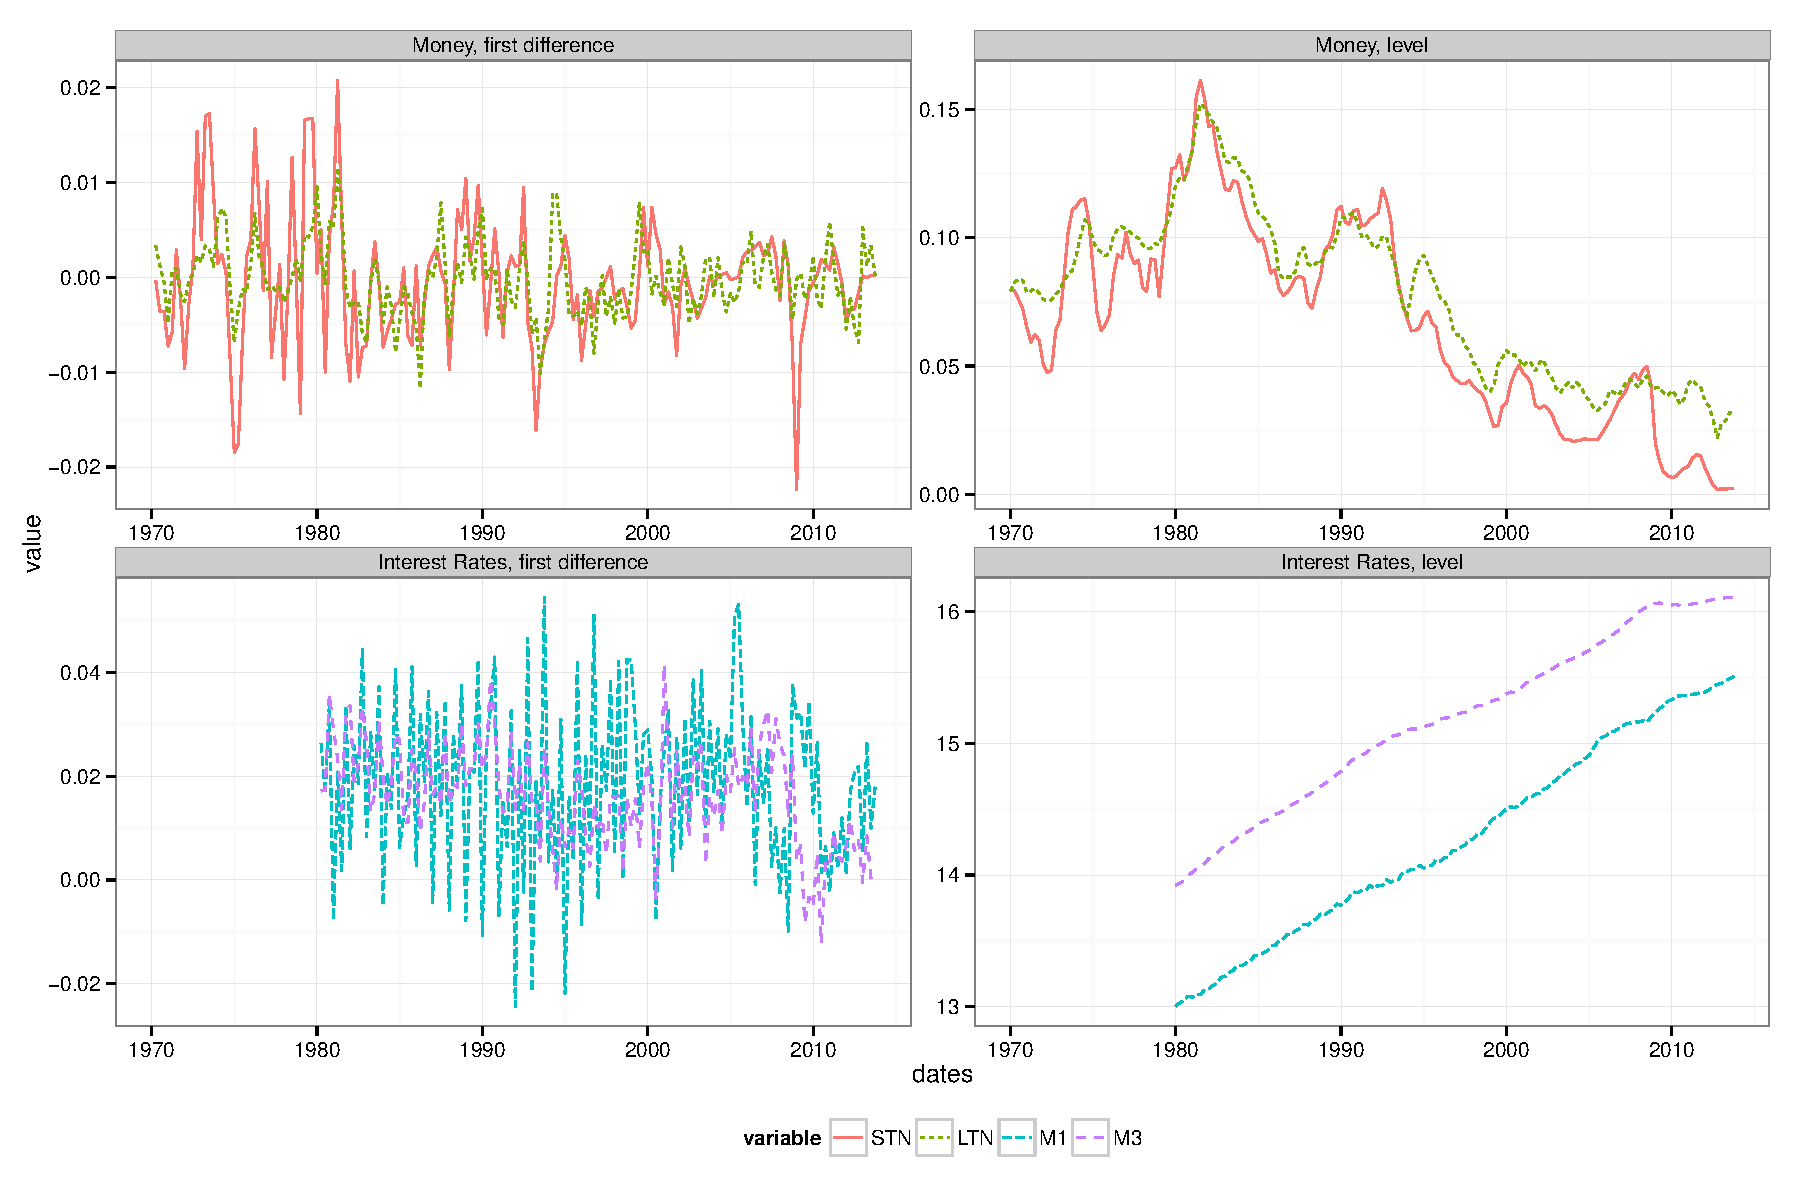
\includegraphics[width=\textwidth]{figure/plot_moneyir-1} 

}



\end{knitrout}

Strong seasonal effect in M1, M3 seems better behaved. 


\begin{knitrout}
\definecolor{shadecolor}{rgb}{0.969, 0.969, 0.969}\color{fgcolor}

{\centering 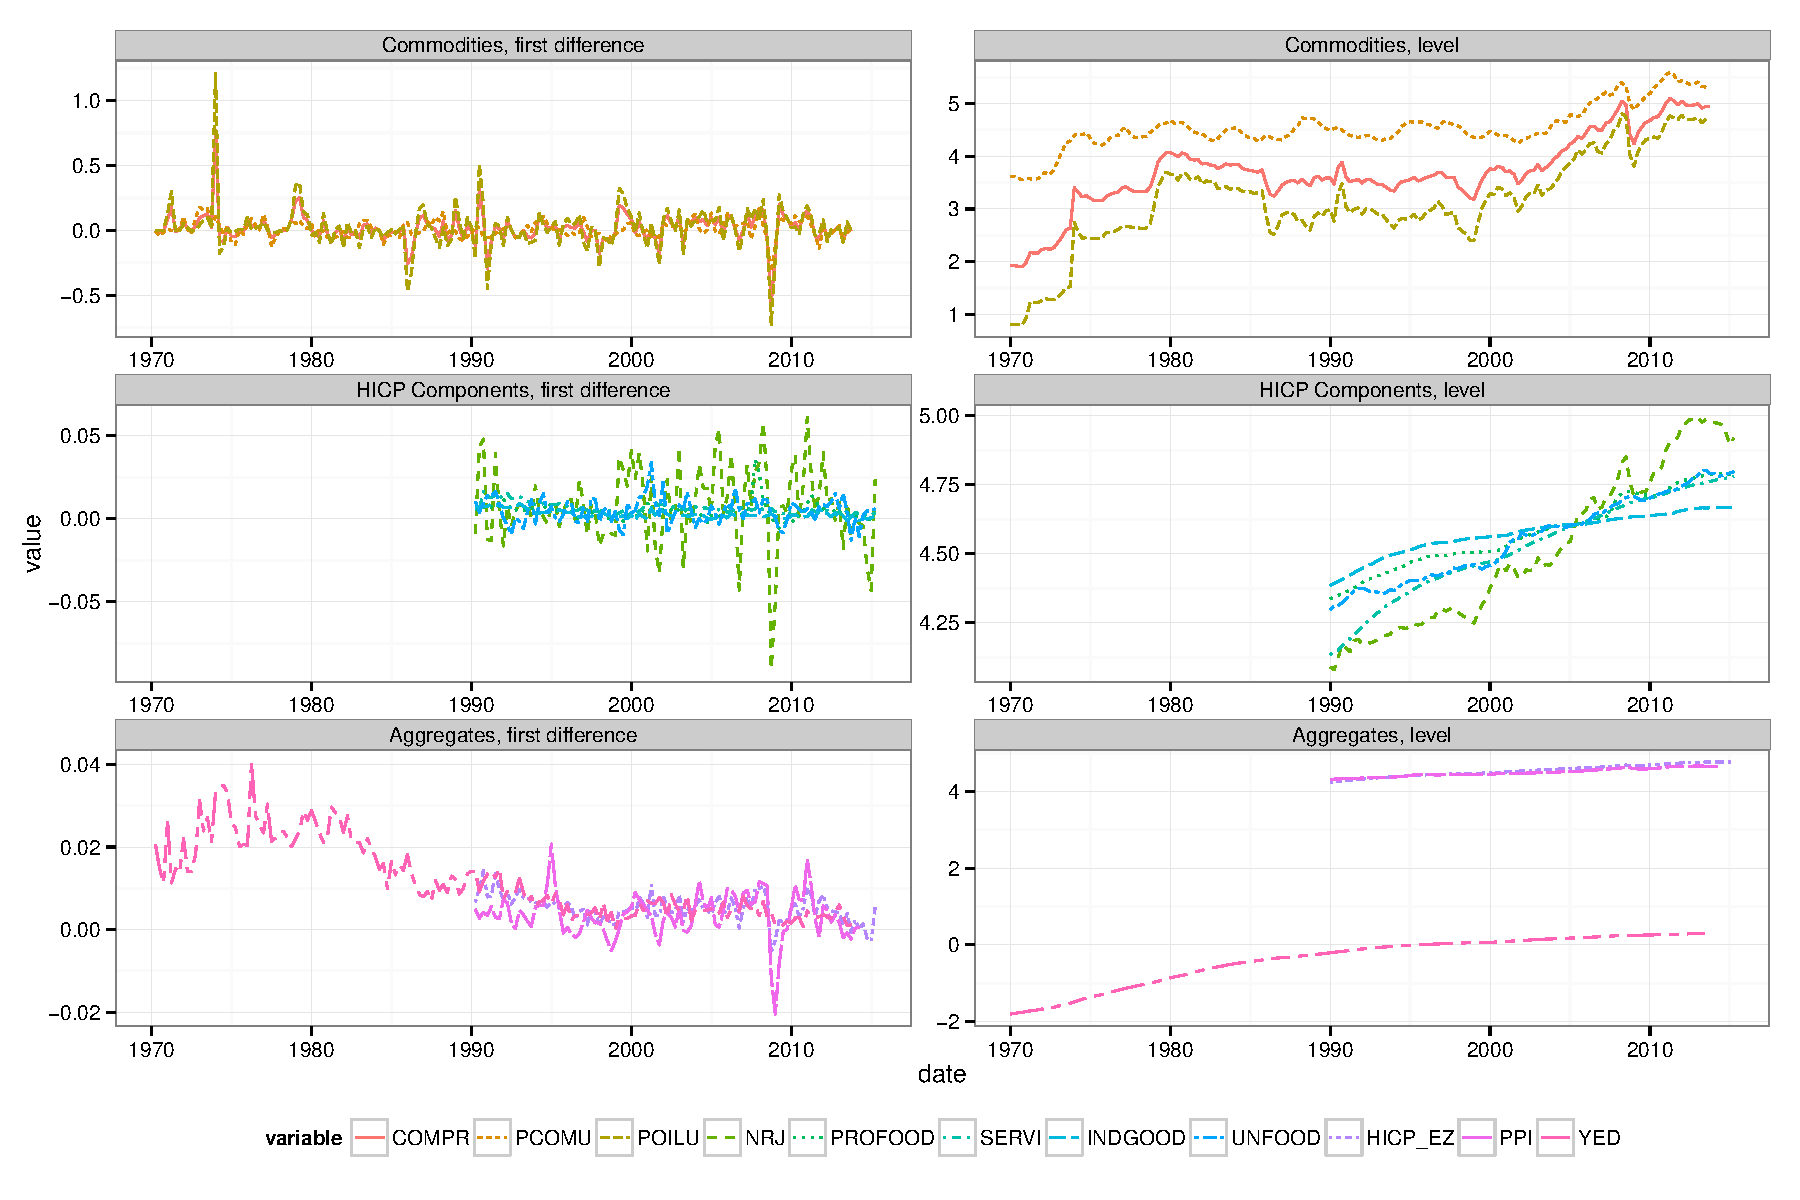
\includegraphics[width=\textwidth]{figure/plot_price-1} 

}



\end{knitrout}




\begin{knitrout}
\definecolor{shadecolor}{rgb}{0.969, 0.969, 0.969}\color{fgcolor}

{\centering 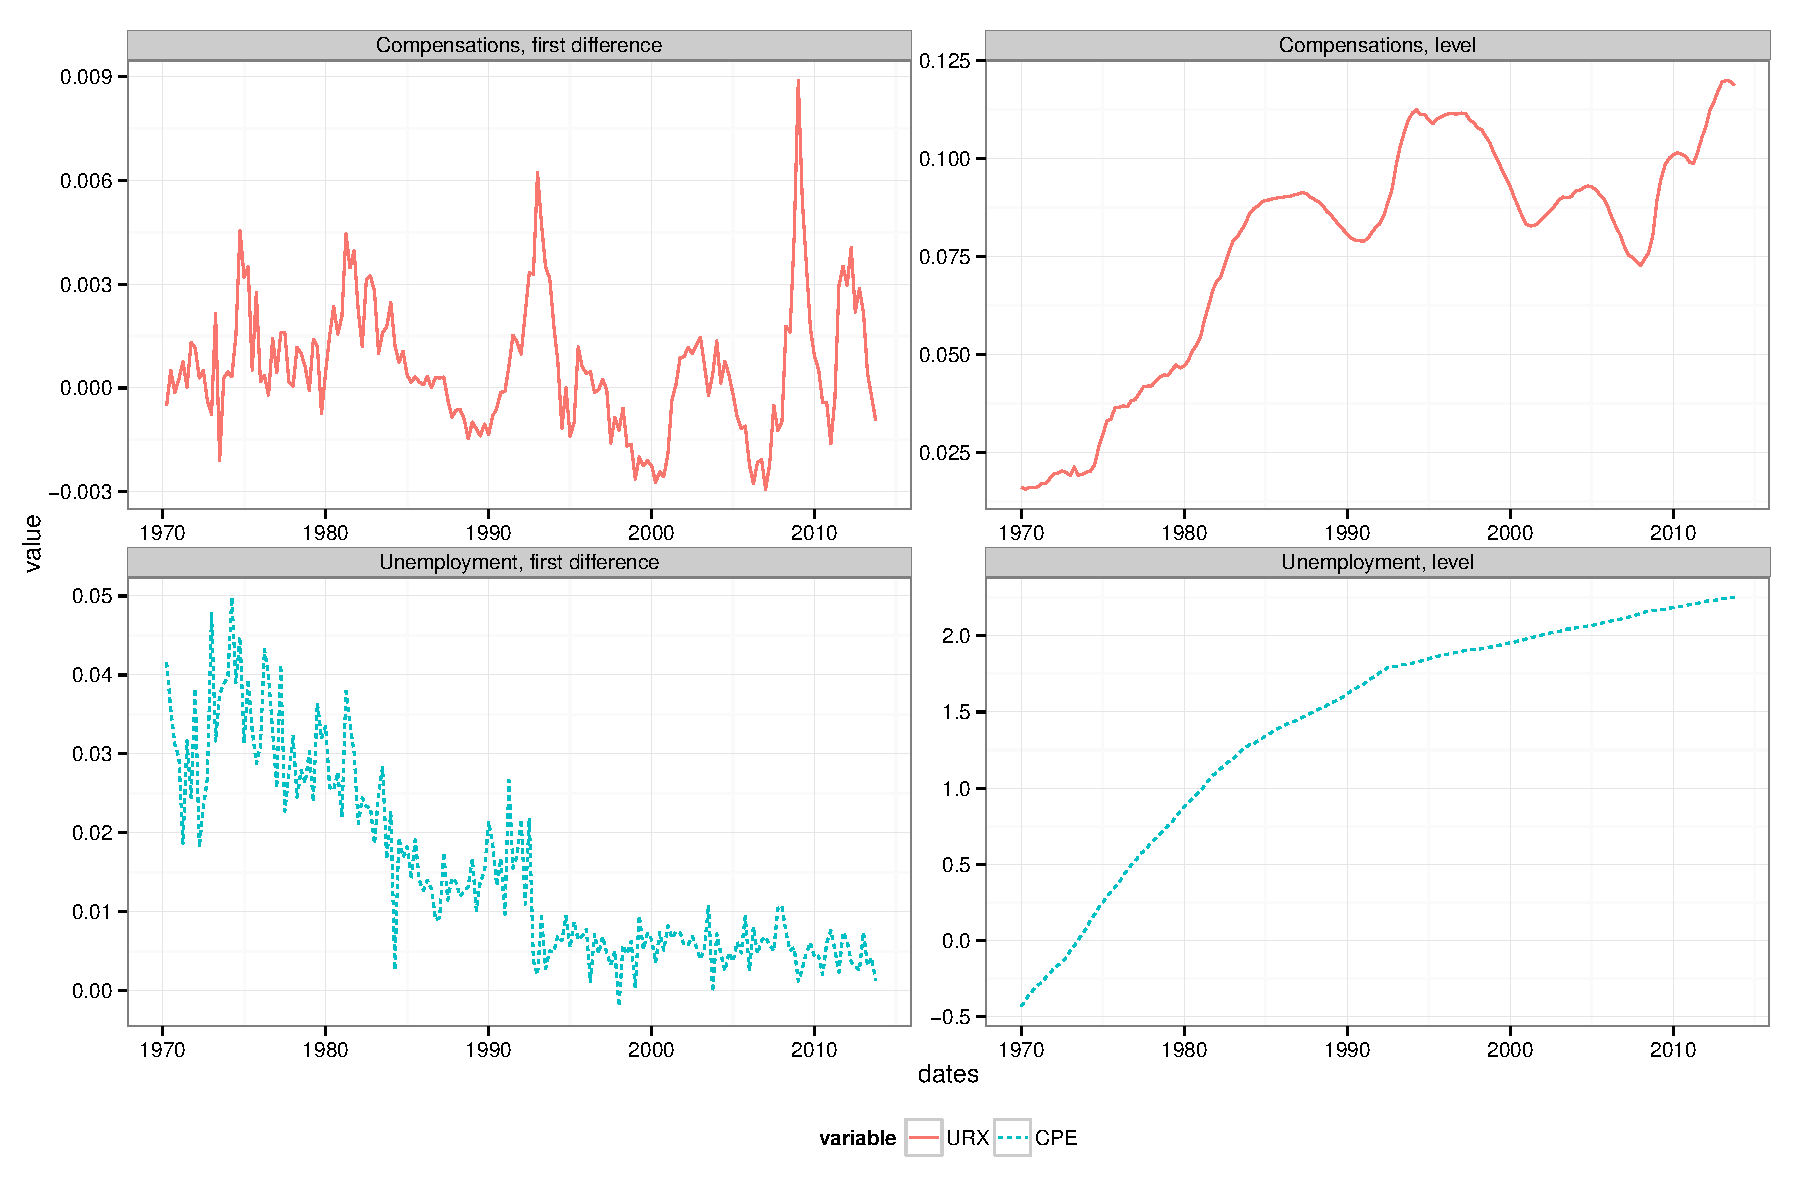
\includegraphics[width=\textwidth]{figure/plot_cou_uem-1} 

}



\end{knitrout}



\begin{knitrout}
\definecolor{shadecolor}{rgb}{0.969, 0.969, 0.969}\color{fgcolor}

{\centering 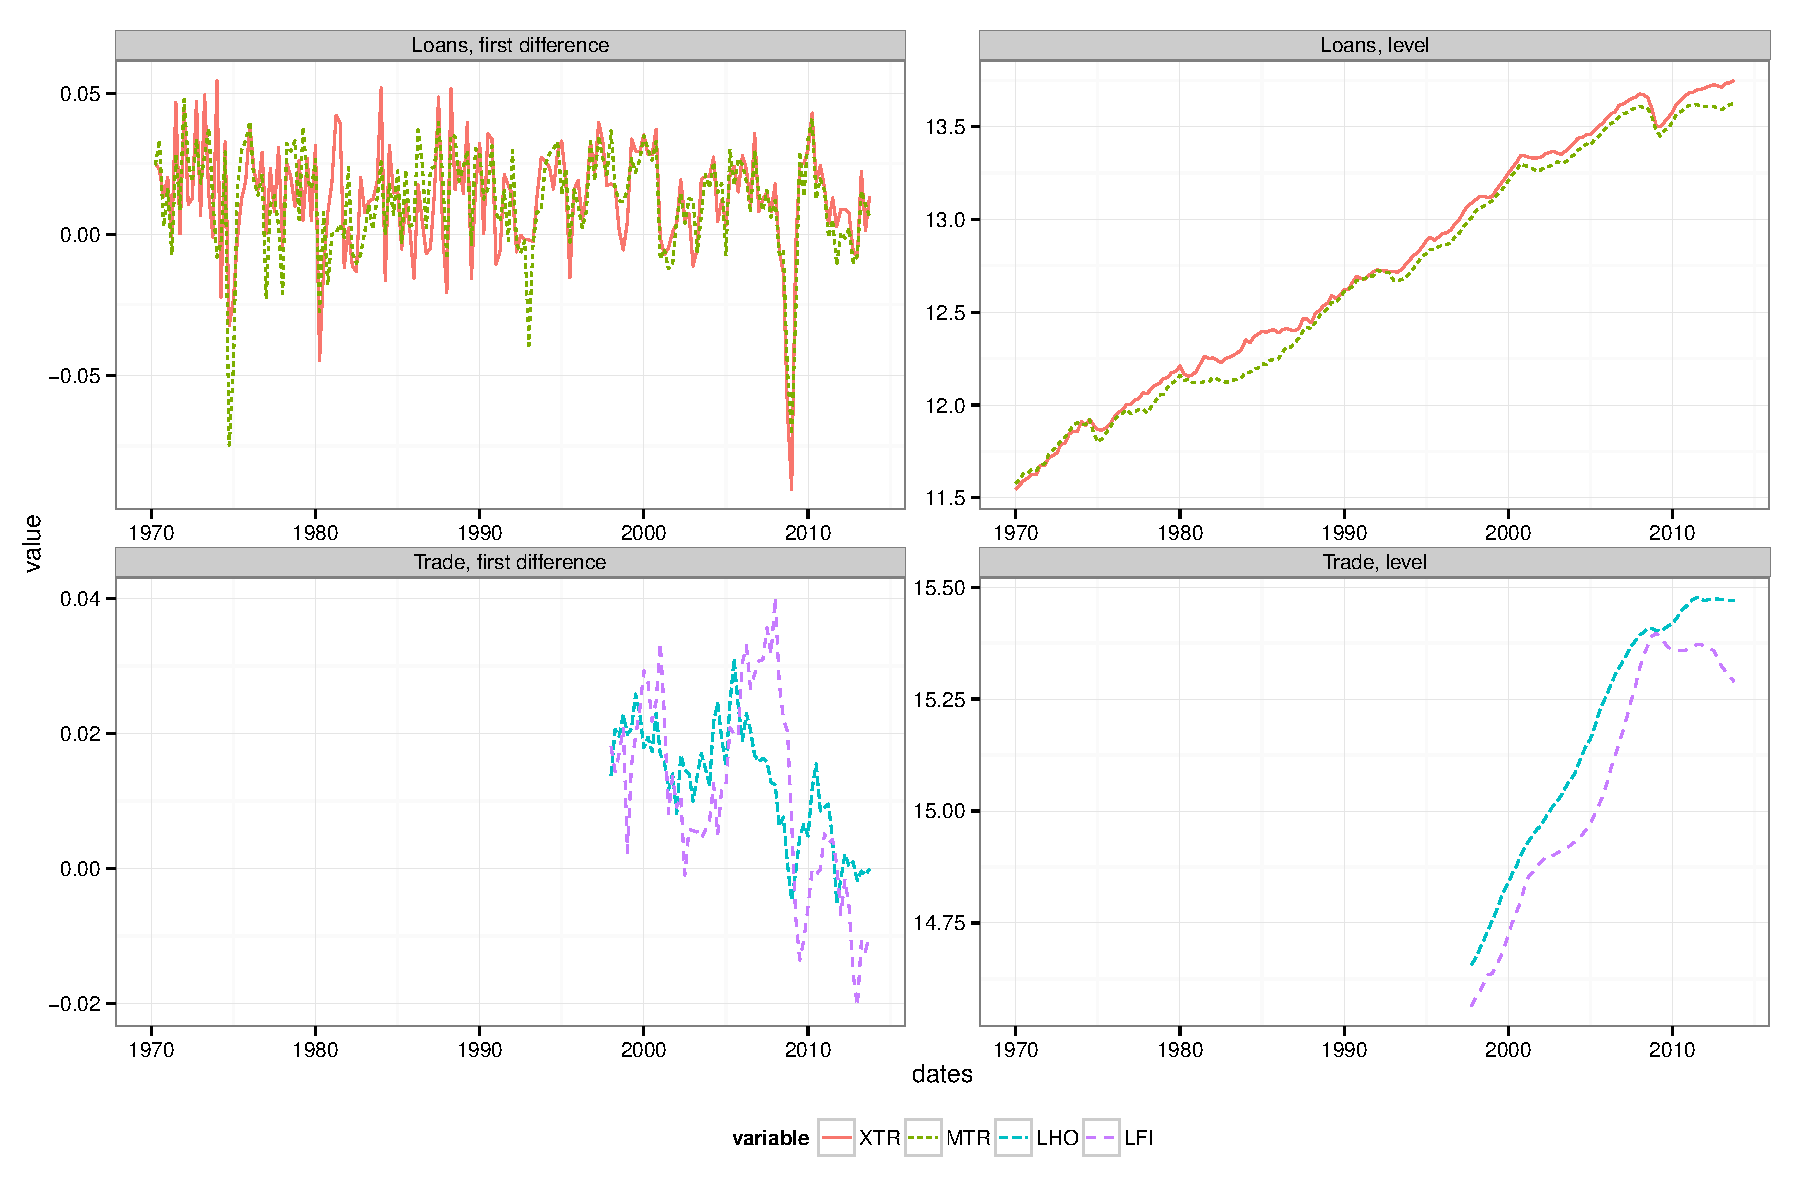
\includegraphics[width=\textwidth]{figure/plot_rest-1} 

}



\end{knitrout}

\clearpage
\newpage

\section{Money demand function}

\cite{baardsen2005econometrics} estimates a money demand function on AWM data from 1980:4 to 1997:2. The equation is based on a model from \cite{coenen2001demand} and it includes lagged and contemporanous variables as well as an error correction term. It has the form:
\begin{align*}
\Delta \widehat{\left(m-p\right)_t} &= \alpha_0 + \alpha_1 \Delta \Delta y_t + \alpha_2 \frac{\Delta RS_t + \Delta RS_{t-1}}{2} 
+ \alpha_3 \Delta RL_{t-1} \\
&+ \alpha_4 \frac{\Delta pan_t + \Delta pan_{t-1}}{2} + \alpha_5 emc_{t-2},\\
ecm_t &= (m-p)_t + \beta_1 y_t + \beta_2 \Delta pan_t + \beta_3 (RL-RS)_t.
\end{align*}

The \text{it} is a co-intergration relation taken form references in \cite[p. 152]{baardsen2005econometrics}. $RL$ and $RS$ are the short and long rates from the AWM, $y_t$ the log of real GDP, and $\Delta pan$ is the annualized change in the GDP deflator.  

Let's try to estimate some variation of it. We do not include an ECM term for starters, and the GDP deflator isn't in the data yet. 
\begin{knitrout}
\definecolor{shadecolor}{rgb}{0.969, 0.969, 0.969}\color{fgcolor}\begin{kframe}
\begin{verbatim}
## 
## Call:
## lm(formula = dmp ~ L1_dmp + ddy + LD0_STN + LD1_STN + LD2_STN + 
##     LD0_LTN + LD1_LTN + LD2_LTN, data = cbind(awm, LD))
## 
## Residuals:
##       Min        1Q    Median        3Q       Max 
## -0.021360 -0.006772 -0.001146  0.005768  0.024458 
## 
## Coefficients:
##              Estimate Std. Error t value Pr(>|t|)    
## (Intercept)  0.005526   0.002586   2.137 0.035517 *  
## L1_dmp       0.347456   0.099563   3.490 0.000773 ***
## ddy          0.222234   0.196361   1.132 0.260954    
## LD0_STN     -0.818803   0.358442  -2.284 0.024874 *  
## LD1_STN      0.732357   0.402077   1.821 0.072101 .  
## LD2_STN      0.105485   0.393424   0.268 0.789264    
## LD0_LTN     -0.188801   0.271217  -0.696 0.488272    
## LD1_LTN      0.334666   0.303381   1.103 0.273124    
## LD2_LTN      0.404098   0.252506   1.600 0.113276    
## ---
## Signif. codes:  0 '***' 0.001 '**' 0.01 '*' 0.05 '.' 0.1 ' ' 1
## 
## Residual standard error: 0.008809 on 84 degrees of freedom
##   (83 observations deleted due to missingness)
## Multiple R-squared:  0.2465,	Adjusted R-squared:  0.1747 
## F-statistic: 3.435 on 8 and 84 DF,  p-value: 0.00182
## Call:
## lassovar(dat = var1, lags = 4)
## 
## Model estimated equation by equation
## Selection criterion: BIC
## Estimator: Lasso
## Deterministics: intercept.
## Dimensions: T = 91  N = 4
## 
## Total number of variables selected:20 (31.25% of candidates)
## 
##  Model summary statistics:
##                  Lambda non-zero    resid var
## dmp        0.0004031671       10 4.880706e-05
## LD0_HICPSA 0.0005798616        3 9.937317e-06
## LD0_STN    0.0005322228        2 6.832299e-06
## LD0_LTN    0.0003189406        5 1.125708e-05
## 
## Deterministics not included in the non-zero count.
##                       [,1]          [,2]        [,3]          [,4]
##                0.002327635 -0.0007433861 0.003219391  5.438899e-05
## 1L_dmp         0.055006039  0.0000000000 0.000000000  0.000000e+00
## 1L_LD0_HICPSA -0.141505112  0.2452826138 0.000000000  2.714080e-01
## 1L_LD0_STN     0.000000000  0.0000000000 0.240385061  2.510174e-01
## 1L_LD0_LTN     0.444229932  0.0000000000 0.000000000  3.663671e-01
## 2L_dmp         0.082117048  0.0000000000 0.000000000  0.000000e+00
## 2L_LD0_HICPSA  0.000000000  0.0000000000 0.000000000  0.000000e+00
## 2L_LD0_STN     0.000000000  0.0000000000 0.000000000 -1.811055e-01
## 2L_LD0_LTN     0.181701749  0.0000000000 0.000000000  0.000000e+00
## 3L_dmp         0.000000000  0.0000000000 0.000000000  0.000000e+00
## 3L_LD0_HICPSA -0.295219256  0.0000000000 0.000000000  0.000000e+00
## 3L_LD0_STN     0.000000000  0.0000000000 0.155102212  0.000000e+00
## 3L_LD0_LTN     0.174285594  0.0000000000 0.000000000  0.000000e+00
## 4L_dmp         0.450750917  0.0000000000 0.000000000  0.000000e+00
## 4L_LD0_HICPSA  0.000000000 -0.0523451587 0.000000000  0.000000e+00
## 4L_LD0_STN     0.250079448  0.0000000000 0.000000000 -1.632384e-01
## 4L_LD0_LTN     0.308291408 -0.0803711365 0.000000000  0.000000e+00
\end{verbatim}
\end{kframe}
\end{knitrout}


Some models in levels:
\begin{knitrout}
\definecolor{shadecolor}{rgb}{0.969, 0.969, 0.969}\color{fgcolor}\begin{kframe}
\begin{verbatim}
## 
## Call:
## lm(formula = mp ~ YER + STN + LTN, data = awm)
## 
## Residuals:
##      Min       1Q   Median       3Q      Max 
## -0.11779 -0.03585 -0.00800  0.03598  0.15127 
## 
## Coefficients:
##             Estimate Std. Error t value Pr(>|t|)    
## (Intercept) -25.0117     1.8767 -13.327  < 2e-16 ***
## YER           2.5007     0.1291  19.364  < 2e-16 ***
## STN          -1.8992     0.6127  -3.100  0.00257 ** 
## LTN           4.3620     1.0428   4.183 6.56e-05 ***
## ---
## Signif. codes:  0 '***' 0.001 '**' 0.01 '*' 0.05 '.' 0.1 ' ' 1
## 
## Residual standard error: 0.06377 on 92 degrees of freedom
##   (80 observations deleted due to missingness)
## Multiple R-squared:  0.9441,	Adjusted R-squared:  0.9423 
## F-statistic: 517.8 on 3 and 92 DF,  p-value: < 2.2e-16
##                    [,1]
##            1.3388037179
## 1L_dat     0.8765929977
## STN        0.0000000000
## LTN        0.0000000000
## YER        0.0003278016
## LD0_HICPSA 0.0000000000
##                     [,1]         [,2]        [,3]        [,4]
##               -1.1960265  0.042599060  0.18303063  0.76113369
## 1L_mp          0.9257880 -0.003811509  0.00000000  0.00000000
## 1L_STN         0.0000000  0.945491666  0.04670236 -0.10497598
## 1L_LTN         0.0000000  0.005022450  0.85051184 -0.06335923
## 1L_YER         0.1407295  0.000000000 -0.01241340  0.94748692
## 1L_LD0_HICPSA  0.0000000  0.504065809  0.43919307  0.33430108
##                        [,5]
##                0.0008704405
## 1L_mp          0.0000000000
## 1L_STN         0.0000000000
## 1L_LTN        -0.0246811771
## 1L_YER         0.0000000000
## 1L_LD0_HICPSA  0.3564794659
\end{verbatim}
\end{kframe}
\end{knitrout}
Totally different from the relation in JAE/Baardsen, but then again the modes are totally difference as well.

\section{Inflation models}







\clearpage
\newpage

\bibliographystyle{chicagoa}
\bibliography{bib}

\end{document}
